\chapter{Implementation}
In this chapter I will discuss why it is interesting to implement AD in Julia. I will also give some implementation specific details and benchmark the implementation against other AD libraries in Julia and MATLAB.
\label{ch:Implementation}
\section{Julia}
\label{sec:Julia}
Julia is a new programming language that was created by Jeff Bezanson, Alan Edelman, Stefan Karpinski and Viral B. Shah at MIT, Massachusetts Institute of Technology \emph{\citep{juliaLab}}. The language was created in 2009, but was first released publicly in 2012. In 2012 the creators said in a blog post that:
\begin{quotation}
"We want a language that’s open source, with a liberal license. We want the speed of C with the dynamism of Ruby. We want a language that’s homoiconic, with true macros like Lisp, but with obvious, familiar mathematical notation like Matlab. We want something as usable for general programming as Python, as easy for statistics as R, as natural for string processing as Perl, as powerful for linear algebra as Matlab, as good at gluing programs together as the shell. Something that is dirt simple to learn, yet keeps the most serious hackers happy. We want it interactive and we want it compiled. (Did we mention it should be as fast as C?)"\emph{\citep{juliaBlogRelease2012}}.
\end{quotation}
In short, it seems to be the perfect language for numerical applications and it would be interesting to see how it performs compared to MATLAB. When it comes to AD in Julia, there are already some packages that can be used. Most of them are backward AD-packages designed for machine learning, for example AutoGrad \emph{\citep{knet2016mlsys}} and Zygote \emph{\citep{innes2018don}}. The reason why AD-packages for machine learning are based on backward AD is that, without going to deep into the subject, it largely consist of minimization of functions with a large number of input parameters, but with only one output parameter. As discussed in \autoref{sec:BackwardAD}, backward AD is much more efficient than forward AD in these types of evaluations. For numerical applications there is usually many input parameters and output parameters. Hence there is no clear advantage of using backward AD compared to forward AD. In Julia there is one package called \textit{ForwardDiff} \emph{\citep{ForwardDiff}} that uses forward AD, being developed by the Julia community. ForwardDiff uses dual numbers as explained in \autoref{sec:DualNumbers} extended to multiple dimensions. This is called multidimensional dual numbers and a vector \textbf{x} of length $n$ is represented as
\begin{align*}
    \textbf{x} = \begin{bmatrix}
    x_1 + \epsilon_1 \\
    \vdots \\
    x_i + \epsilon_i \\
    \vdots \\
    x_n + \epsilon_n \\
    \end{bmatrix}.
\end{align*}
 This package works very well for some applications, but for especially numerical applications it has some limitations that are not ideal, for example: 
\begin{itemize}
    \item The function we want to differentiate only accepts a single argument. This is possible to work around -- if you have vector function $f$ with input parameters $x,y,z \in \Re^n$, you can merge them into one vector of length $3n$ and then obtain the Jacobian. Although this works and you get the correct answer, it is not optimal as you would have to make local workarounds to make the code work, causing unreadable code.
    \item The function we want to differentiate must be on the form of a generic Julia function, such as: $g(x) = 3x*x$. Here $x*x$ symbolize element-wise multiplication. This means that if we have a function like $h(x) = 3x*x + \text{sum}(x)$, where all elements in $g(x)$ are added with the sum of all elements in $x$, it will not be possible to use \textit{ForwardDiff} to obtain the Jacobian. This limitation also prevents us from having a function that we evaluate for all points, and then add boundary conditions for some points later. This is a feature that is essential for most numerical analysis.
    \item The Jacobian calculated by \textit{ForwardDiff} is a full matrix. In some calculations when the Jacobian is dense anyway, this will not have any major adverse effects, but in many numerical applications, the Jacobian will be sparse. By representing a sparse matrix on a full matrix format, a lot of potential computation efficiency is lost.
\end{itemize}

\section{Implementation of Automatic Differentiation}
\label{sec:ImplementationAD}
When it comes to efficiently implementing AD, there are two factors to consider. Firstly, it must be easy and intuitive to use. Secondly, it must be efficient code as it will be used in computational demanding calculations. A convenient way to store the AD-variables in Julia is to make a structured array (\texttt{struct}) that has two member variables, \texttt{val} and \texttt{jac}, that stores respectively the value and the corresponding Jacobian: 
\lstinputlisting{code/AD_struct.jl} 
The \texttt{val} variable is a vector with elements of type \texttt{Float64}. If the AD-variable is only a scalar, then the implementation can either stick to \texttt{val} being a vector, only of length one, or it can be just a scalar in this specific case. The option where \texttt{val} always is a vector is most consistent and can avoid possible problems that can occur when we do not know what types the AD struct contains at different times. When it comes to the Jacobian, there are multiple ways of storing the matrix. Depending on the application, how much, and what type of manipulation of the matrix you are going to do, the choice is based on efficiency and convenience. I will describe two different methods on how to store the Jacobian. Both implementations are inspired by two different implementations in MRST \emph{\citep{lieMrstUrl}}. In the first implementation the Jacobian, \texttt{jac}, is represented as a vector of sparse matrices. Each element in the vector is a sparse matrix that represent the Jacobian w.r.t. each primary variable. This implementation gives the freedom to easily work with the Jacobian for just a single primary variable. Before introducing the second implementation of the Jacobian, I will continue to explain the implementation of what I will call \texttt{ForwardAutoDiff}(\texttt{FAD}), which is defined with the following struct:
\lstinputlisting{code/FADStruct.jl}


To obtain a working AD library we need to implement operators for the \texttt{FAD} struct. The importance of the way you implement the AD operators and elementary functions can be expressed in a short example: Assume you have two \texttt{FAD} variables $x$ and $y$ and that you want to compute the function $f(x,y) = y+\exp(2xy)$. If the implementation is based on making new functions that take in \texttt{FAD}-variables as input parameters, it will for the evaluation of $f$ look something like this: 
\begin{center}
    $f$ = \texttt{FADplus}($y$,\texttt{FADexp}(\texttt{FADtimes}(2,\texttt{FADtimes}($x,y$)))).
\end{center}
This is clearly not a suitable way to implement AD as it quickly becomes difficult to see what type of expression it is. If you did not know what type of function f is, it would take you quite some time to figure it out. And more importantly, the possibility for human error becomes very large when you have to write unreadable code like this. This approach should be avoided. Lie and Neidinger suggests in \emph{\cite{lieMrstUrl}} and \emph{\cite{doi:10.1137/080743627}} a much more elegant implementation, where instead of making new functions that take in \texttt{FAD}-variables as parameters, one should overload the standard operators (+,-,*,/) and the elementary functions (exp, sin, log, etc.). This is where the elegance of having a custom \texttt{FAD} struct. In Julia we can use \emph{multiple dispatch} to call our implementation of standard operators and elementary functions when they are used on \texttt{FAD} structs. A quick explanation of \emph{multiple dispatch} that satisfies our needs is that at runtime, the compiler understands what types are given as input for either an operator or a function and chooses the correct method based on this. To demonstrate, this is done by implementing a function \lstinputlisting{code/overload_plus_operator_AD.jl} 
that overloads the + operator. Here, we import the + operator from Base (which is where the standard functions in Julia lie) and overload it for \texttt{FAD} variables. For compactness purposes I have removed checks and edge cases and only left the method for \texttt{FAD} variables with equal length. The broadcast function add each Jacobian for each primary variable together. This implementation of the + operator is only used when there are \texttt{FAD} variables on both sides of the operator. Hence, if $x = 1$, $y = 3$ and then $z = x+y$ is computed, Julia understands that it is not the definition above, but the normal addition for integers it should use. But if $x,y = \texttt{initialize\_FAD}(1,3)$ is declared, so that $x$ and $y$ both are \texttt{FAD} variables, then Julia's multiple dispatch will understand that the new definition of the "+"-operator should be used on the expression $z = x+y$. What we need to remember is that if I now write $z = x + 3$, with $x$ as an \texttt{FAD} variable, Julia will deploy an error message. This is because we also have to implement
\lstinputlisting{code/overload_plus_operator_number.jl}
Here, the first function will be used if the + operator is used with an \texttt{FAD} variable on the left hand side and a number on the right. The last line is a compact way of writing the opposite function, which will be used when the number is on the right hand side. When we have implemented all the functions necessary, it gives us the opportunity for the function $f$ above to simply write $f = y+\exp(2*x*y)$ and Julia will understand that it is our implementation of + and * operators and the exponential function that shall be used. $f$ will now become an \texttt{FAD}-variable with the correct value and derivatives. 

Up until now I have only discussed implementation of \texttt{FAD} for scalar variables. But another advantage of Julia's multiple dispatch system is clear if we start looking at vector variables and functions. In some situations, like in \autoref{ch:FlowSolver}, we want to sum over all the elements in the vector. If we look at how we can overload the \texttt{sum} function one might think that we would try something like
\lstinputlisting{code/overload_sum.jl}
which would indeed work, a more elegant approach that fully exploit Julia's multiple dispatch, would be to overload the \texttt{iterate} function. This function explains how we shall iterate through an AD variable: 
\lstinputlisting{code/iterate.jl}
Now, the built-in \texttt{sum} function will work on AD variables since it knows how to iterate through the variables. When it adds up the values, the "+"-operator we defined above is being used. And not only that! All built-in functions that iterate through the input will also work (given that the functions they use on the variable also are overloaded). As an example, if we now overload the division operator as well as the ones talked about above, the Base function \texttt{mean} will also work on \texttt{FAD} variables with no extra work!

\subsection{Element-wise and Vector Multiplication}
When one introduces AD for vectors, one need to discuss how to handle multiplication and division. In mathematical programming languages like MATLAB and Julia, there is a difference between the "*" and ".*" operators. The first operator, "*", is regular vector multiplication, meaning if $v$ is a row vector and $u$ is a column vector, both of length $n$, then $v*u$ is the normal vector product that results in a scalar, and $u*v$ gives an $n\times n$ matrix where each row in $v$ is multiplied by the corresponding row value of $u$. An attempt to evaluate $u*u$ will end in an error message saying that "the dimensions does not match matrix multiplication". The ".*" operator however, is the element-wise multiplication operator. This means that if we have regular column vectors like $u$ and $w = v'$, the transpose of $v$, the evaluation of $u.*w$ will be element-wise multiplication of $u$ and $w$, into a new vector of same dimensions as $u$ and $w$. Here one need to make a choice in the implementation of multiplication and division for AD in Julia, because as of now, there are no good ways of overloading any dot operators for custom types such as AD. The Julia issue \emph{\cite{JuliaIssueDot}} from 2017 explains the problems of overloading the element-wise ".*" operator, and that there is no good way of actually doing this. The issue has still not been resolved. With this in mind, and that there will only be used element-wise multiplication in this project, I have decided to implement "*" as element-wise multiplication. This means that if I have written regular multiplication expressions consisting of at least one AD-variable, it is element-wise multiplication that is being executed.

\subsection{Optimizing \texttt{ForwardAutoDiff}}
By looking closer at the implementation of the Jacobian in \texttt{FAD} we can find that in some cases there are better approaches to storing the Jacobian that will gain computational efficiency. Before looking closer at the specific situations, I will explain how the sparse matrix type, \texttt{SparseMatrixCSC}, that \texttt{FAD} uses is built up and how it works. \texttt{SparseMatrixCSC} stands for \textit{Compressed Sparse Column Sparse Matrix Storage} and according to Julia docs \emph{\citep{SparseMatrixCSC}} the SparseMatrixCSC struct is given as
\lstinputlisting{code/SparseMatrixCSCStruct.jl}
It represents a matrix with three vectors and two integers. The integers represents the size of the matrix and the three vectors represents all non-zero elements in the matrix. Two explain how the vectors work, consider the example of a matrix \textbf{A} with the corresponding \texttt{SparseMatrixCSC} struct variables:
\begin{multicols}{2}
    \begin{align*}
        \textbf{A} = \begin{pmatrix}
        1&0&0&5&0\\
        0&3&0&6&0\\
        0&0&0&0&7\\
        2&4&0&0&0\end{pmatrix}
    \end{align*}
    \columnbreak
    \begin{align*}
        \texttt{m} &= 4\\
        \texttt{n} &= 5\\
        \texttt{colptr} &= [1, 3, 5, 5, 7, 8]\\
        \texttt{rowval} &= [1, 4, 2, 4, 1, 2, 3]\\
        \texttt{nzval} &= [1, 2, 3, 4, 5, 6, 7].
    \end{align*}
\end{multicols}
\texttt{nzval} contains all the non-zero elements in \textbf{A}. The order of the numbers is given by column from left to right and then row from top to bottom. \texttt{rowval} has the same ordering as \texttt{nzval} and gives the row number to the corresponding value in \texttt{nzval}. \texttt{colptr} contains the information of how many non-zero numbers there are in each column. For column number $i$, the sequence \texttt{colptr}$[i]$:\texttt{colptr}$[i+1]-1$ gives the indices in \texttt{nzval} and \texttt{rowval} that corresponds to values in this column. For matrix A and column number 2 we get the indices
\begin{equation*}
    \texttt{colptr}[2]:(\texttt{colptr}[3]-1) \Longrightarrow 3:4,
\end{equation*}
which gives row number 2 and 4 and values 3 and 4. For a column with only zero elements, like column 3, the sequence becomes
\begin{equation*}
    \texttt{colptr}[3]:(\texttt{colptr}[4]-1)\Longrightarrow 5:4,
\end{equation*}
which indicates that there are no non-zero elements in this column. 

This way of storing a matrix will decrease both memory usage and computational efficiency dramatically when working with large and sparse matrices compared to storing the full matrix. When performing operations on the matrix, e.g. an element-wise vector matrix  multiplication, the computational gain comes from the opportunity to neglect all zero values. If we store the matrix as a full dense matrix then we have to compute a lot of multiplications that ends up being zero that we with a sparse matrix structure could avoid computing. The method however brings some extra work that consist of doing numerous checks to make sure that we have done the multiplication correctly. Take the example from \autoref{sec:FADWithMultipleParameters} where $f = 2\cdot \textbf{x}\cdot \textbf{y}$ for the primary variables $\textbf{x},\textbf{y}\in \Re^3$ as in Definition \eqref{def:VectorAD}. Initializing the primary variables as \texttt{FAD}-structs gives 
\begin{multicols}{2}
    \noindent
    \begin{align*}
        \textbf{x} = \left[\adpair{\begin{pmatrix}1\\2\\3
        \end{pmatrix}}{\left\{\adpair{
        \begin{pmatrix}
        1&0&0\\
        0&1&0\\
        0&0&1\end{pmatrix}}
        {\begin{pmatrix}
        0&0&0\\
        0&0&0\\
        0&0&0
        \end{pmatrix}}\right\}} \right]
    \end{align*}
    \begin{align*}
        \textbf{y} = \left[\adpair{\begin{pmatrix}4\\5\\6
        \end{pmatrix}}{\left\{\adpair{
        \begin{pmatrix}
        0&0&0\\
        0&0&0\\
        0&0&0\end{pmatrix}}
        {\begin{pmatrix}
        1&0&0\\
        0&1&0\\
        0&0&1
        \end{pmatrix}}\right\}} \right].
    \end{align*}
\end{multicols}
Here I have written out the Jacobians as full matrices for better visualization although in theory they will be stored as \texttt{SparseMatrixCSC} structs. In the multiplication of the two \texttt{FAD}-variables, the element-wise multiplication of the values are not interesting and we will focus on how we obtain the new Jacobian for $\textbf{x}\cdot \textbf{y}$. Similarly as in \autoref{sec:FADWithMultipleParameters} we find the new Jacobian using the product rule, but now we can separate the operations into two calculations. First we have the Jacobian for the primary variable \textbf{x}:
\begin{align*}
    \begin{pmatrix}
        4&0&0\\
        0&5&0\\
        0&0&6\end{pmatrix}
        \cdot
        \begin{pmatrix}
        1&0&0\\
        0&1&0\\
        0&0&1
        \end{pmatrix}
        +
        \begin{pmatrix}
        1&0&0\\
        0&2&0\\
        0&0&3
        \end{pmatrix}
        \cdot
        \begin{pmatrix}
        0&0&0\\
        0&0&0\\
        0&0&0
        \end{pmatrix}
        \Longrightarrow
        \begin{pmatrix}
        4&0&0\\
        0&5&0\\
        0&0&6
        \end{pmatrix}.
\end{align*}
Then for the primary variable \textbf{y} we obtain the Jacobian
\begin{equation}
    \label{eq:JacobianCalculationY}
    \begin{pmatrix}
        4&0&0\\
        0&5&0\\
        0&0&6\end{pmatrix}
        \cdot
        \begin{pmatrix}
        0&0&0\\
        0&0&0\\
        0&0&0
        \end{pmatrix}
        +
        \begin{pmatrix}
        1&0&0\\
        0&2&0\\
        0&0&3
        \end{pmatrix}
        \cdot
        \begin{pmatrix}
        1&0&0\\
        0&1&0\\
        0&0&1
        \end{pmatrix}
        \Longrightarrow
        \begin{pmatrix}
        1&0&0\\
        0&2&0\\
        0&0&3
        \end{pmatrix}.
\end{equation}
What we immediately observe is that two of the multiplications are unnecessary since one of the matrices are the null matrix. Remember then that the left matrix in all the calculations above actually is a vector that we have transformed into a diagonal matrix to illustrate how the element-wise multiplication happens. This means that when the previous Jacobian is a diagonal matrix, what we actually can do to obtain the new Jacobian, is element-wise multiplication between the vector on the left hand side and the vector that is the diagonal on the Jacobian. And even better, when the previous Jacobian is the identity matrix, like in calculation \eqref{eq:JacobianCalculationY}, the product is simply a diagonal matrix with the left hand side vector on the diagonal. This is where the idea of optimizing \texttt{FAD} comes from. By knowing what type of Jacobian we have at all times we can sometimes take safe shortcuts in our calculations. 

\subsection{Custom Jacobian Automatic Differentiation}
\texttt{Custom Jacobian Automatic Differentiation}(\texttt{CJAD}) is what I have called the optimized \texttt{FAD}. \textit{Custom Jacobian} comes from having four different types of Jacobians. The structure of \texttt{CJAD} is similar to \texttt{FAD}, except that the Jacobians are in a vector of type \texttt{CustomJac}:
\lstinputlisting{code/CJAD-struct.jl}
\texttt{CustomJac} is an abstract type that has four structs that extends it:
\begin{itemize}
    \item \texttt{NullJac} -- a struct only containing two numbers that represents the number of rows and columns.
    \item \texttt{IdentityJac} -- a struct only containing one number that represents the number of rows and columns.
    \item \texttt{DiagJac} -- a struct containing a vector with the diagonal values of the struct. The length of the vector equals the number of rows and columns.
    \item \texttt{SparseJac} -- a struct containing a \texttt{SparseMatrixCSC} matrix.
\end{itemize}
Now it is time for Julia's multiple dispatch to shine. Since Julia understands at runtime what type of \texttt{CustomJac} we have, whether it is a \texttt{NullJac}, \texttt{IdentityJac}, \texttt{DiagJac} or \texttt{SparseJac}, we can implement different methods for all possible combinations. Since we in each implementation know what type of matrix we are dealing with, we can optimize the performance. Take the calculation of the Jacobian w.r.t the primary variable \textbf{y} in \eqref{eq:JacobianCalculationY}. First we have a vector multiplied element-wise by a null matrix. The implementation
\lstinputlisting{code/vectorTimesNullJac.jl}
efficiently knows immidietly that there is no need to do any calculations, the result will be a null matrix of the same size as before. The second calculation is a vector multiplied element-wise by an identity matrix. The result will be a diagonal matrix with the vector on the diagonal. The implementation 
\lstinputlisting{code/vectorTimesIdentityJac.jl}
automatically knows the result of this and makes a diagonal Jacobian with the vector on the left hand side without doing any calculations. Finally we have to add a null matrix and a diagonal matrix, and since there is really no need of doing the adding of zero number, the implementation simply returns the diagonal matrix:
\lstinputlisting{code/nullJacPlusDiagJac.jl}
All the implementations of operators on structs extending the \texttt{CustomJac} type are called from outer functions that check the legality of the operations. Hence there are no checks in the presented implementations.


\section{Benchmarking Automatic Differentiation}
As mentioned in \autoref{sec:Julia}, Julia already has an AD library called \textit{ForwardDiff} \emph{\citep{ForwardDiff}} that uses forward AD. Hence, it would be interesting to see how the different implementations compares when the functions evaluated are getting larger. As another reference, I have added the AD implementation in the MATLAB Reservoir Simulation Toolbox (MRST) \emph{\citep{mrstHomepage}} to the benchmark, to see how the Julia implementations compare to an optimized AD tool in MATLAB. To benchmark the efficiency of the different AD tools, I have evaluated the vector function $f: \Re^{n\times 3} \rightarrow \Re^n $ where
\begin{equation}
\label{eq:benchmarkFunction}
f(x,y,z)  = \exp(2xy) - 4xz^2 + 13x - 7,
\end{equation}
and $x,y,z \in \Re^n$. \autoref{fig:benchmarkAD} shows how computational time for calculating the function value and the Jacobian of the function, for the different methods, scales as the length of the vectors $n$ increases. \footnote{All benchmarks in this project are performed on a MacBook Pro (Retina, 13-inch, Late 2013), 2,8 GHz Intel Core i7 processor and 16 GB 1600 MHz DDR3 memory. For benchmarking time in Julia, I have used the benchmarking library \emph{\cite{BenchmarkTools}}. For benchmarking time in Matlab I have taken the median of mulitple tests using the stopwatch \emph{\cite{TicToc}}.}

\begin{figure}[H]
    \centering
    \begin{subfigure}[t]{0.48\textwidth}
        \centering
        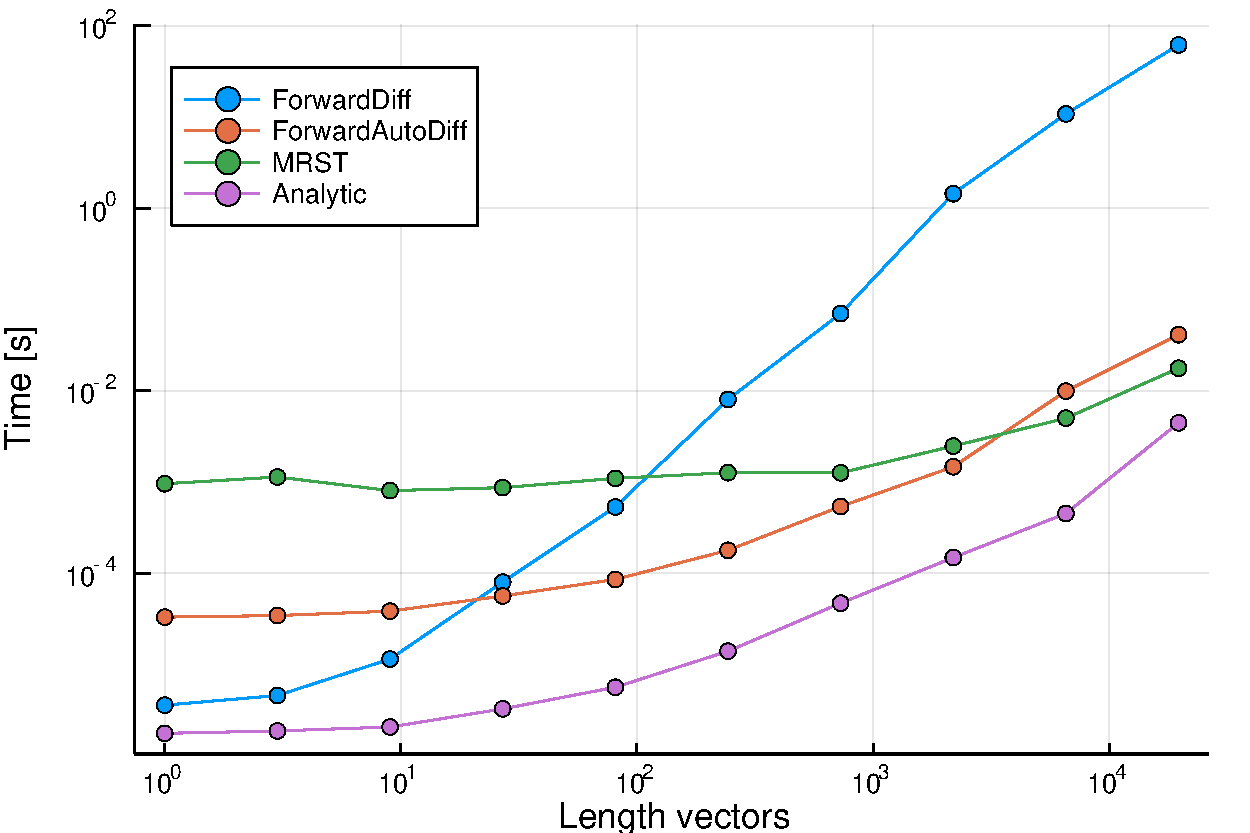
\includegraphics[width = \textwidth]{figures/benchmark_all_ADs.pdf}
        \caption{}
        \label{fig:benchmarkAllADs}
    \end{subfigure}
    \begin{subfigure}[t]{0.49\textwidth}
        \centering
        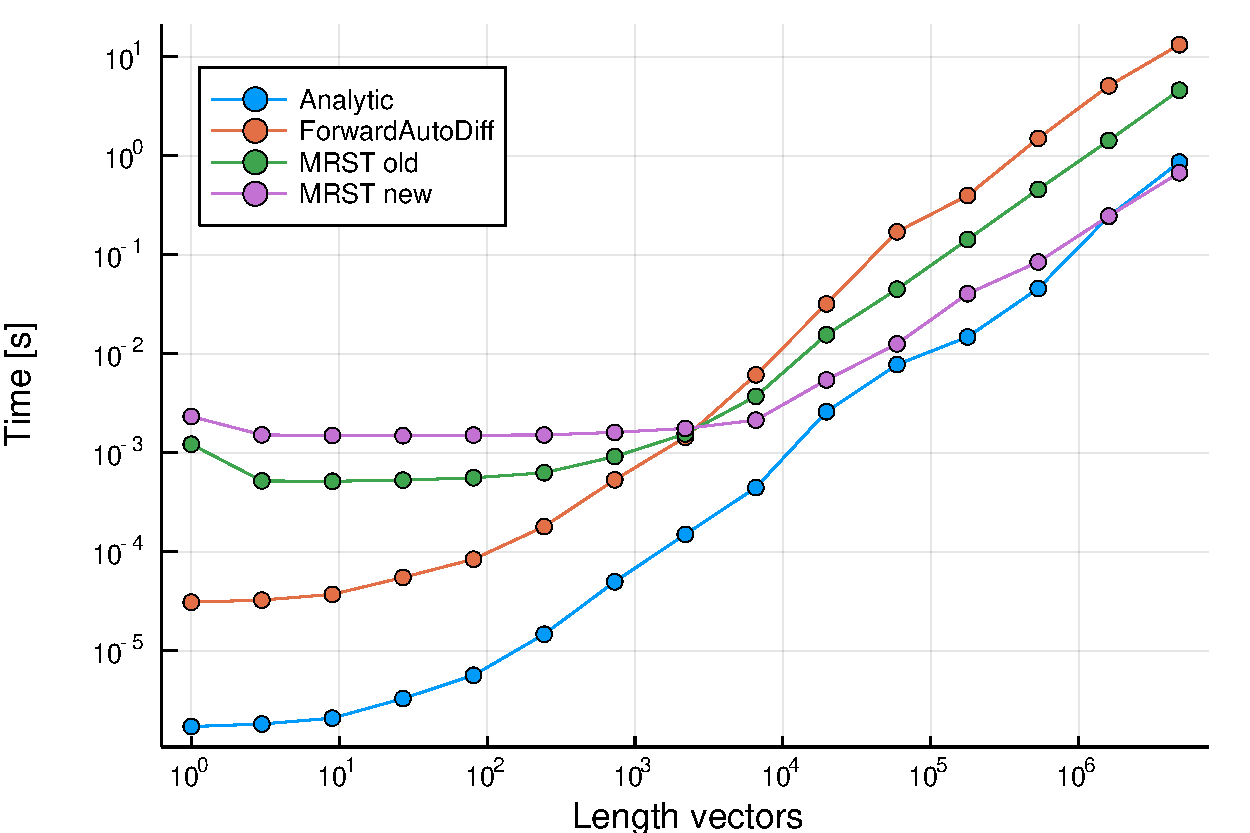
\includegraphics[width = \textwidth]{figures/benchmark_long_vectors_4.pdf}
        \caption{}
        \label{fig:benchmarkLongVectors}
    \end{subfigure}
    \caption{Computational time for calculating the value and Jacobian of $f$ in Equation \eqref{eq:benchmarkFunction} as a function of length of the input vectors.}
    \label{fig:benchmarkAD}
\end{figure}
In \autoref{fig:benchmarkAllADs} we have four different graphs. The analytic graph is simply the evaluation the analytic functions $f(x,y,z)$, $f_x$, $f_y$ and $f_z$. \textit{ForwardDiff} is the AD package in Julia, MRST is the AD tool implemented in MATLAB and \textit{ForwardAutoDiff} is the AD tool I have implemented in Julia. The first thing you observe is that \textit{ForwardDiff} scales very badly as n becomes large. This is because it creates and works with the full Jacobian matrix as discussed in \autoref{sec:Julia}. For $f(x,y,z)$ this will be a $3n \times 3n$ matrix which is a matrix with more than 3 billion elements for the largest values of $n$. We can also observe that for small vectors, MRST and \textit{ForwardAutoDiff} have much more overhead than \textit{ForwardDiff} and the analytic solution. This makes them slower for small $n$, but as $n$ grows, this overhead becomes more negligible. 

The computational costs of both MRST and \textit{ForwardAutoDiff} approach the analytic evaluation as $n$ grows, and it is thus interesting to see how they scale for even larger $n$. This can be seen in \autoref{fig:benchmarkLongVectors}. Here, \textit{ForwardDiff} is left out since it becomes too slow, but I have added a new implementation from MRST, that I will call \textit{MRST new}. The MRST implementation in  \autoref{fig:benchmarkAllADs} is now referred to as \textit{MRST old}. We can observe that the trend seen in \autoref{fig:benchmarkAllADs} where \textit{MRST new} is faster than \textit{ForwardAutoDiff} for vectors longer than 10 000 continues for even longer vectors. As we can see from \autoref{fig:benchmarkLongVectors} \textit{MRST old} is much faster than the two other implementations for long vectors. This is because it is specially optimized for element operations like we have when evaluating the function in Equation \eqref{eq:benchmarkFunction}. \textit{MRST new} exploits that all the Jacobians in the calculation of f simply are diagonal matrices with respect to each primary variable. This means that it can store the values of the diagonals as vectors and calculate the new Jacobians with simple vector multiplication. With this approach we skip the overhead accompanying sparse matrix multiplication. This implementation actually becomes just as fast as the analytic evaluation in Julia for vectors of length $\approx 10^7$. As said, this method is especially efficient for functions like in Equation \eqref{eq:benchmarkFunction}, but if we for example want to calculate something like
\begin{equation}
g(x) = \frac{x\left[2:\text{end}\right] - x\left[1:\text{end}-1\right]}{\texttt{sum(}x\texttt{)}},
\label{eq:differenceFunction}
\end{equation}
the diagonal structure of the Jacobians are gone, and the \textit{MRST new} implementation can not be used. The \textit{MRST old} implementation with the Jacobians as sparse matrices is then used. 

The creators stated in the blog post accompanying the first release of Julia in 2012 \emph{\citep{juliaBlogRelease2012}} that Julia is supposed to be just as fast as C. Hence it would be interesting to see if we can increase, or at least not loose, computational efficiency in the evaluation of the vector function in \eqref{eq:benchmarkFunction} by evaluating it scalar by scalar in a loop instead of by vector multiplications. The difference can be illustrated by the two functions
\lstinputlisting{code/benchmark_functions.jl}
Implementation specific parts are left out. The result can be seen in \autoref{fig:benchmarkADInLoop}, where the graphs with circles as markers are the same methods as in \autoref{fig:benchmarkAllADs} using the function \texttt{benchmarkAD}. The graphs with squares are the same methods, only they are tested with the implementation in function \texttt{benchmarkADinLoop}.
\begin{figure}[H]
    \centering
    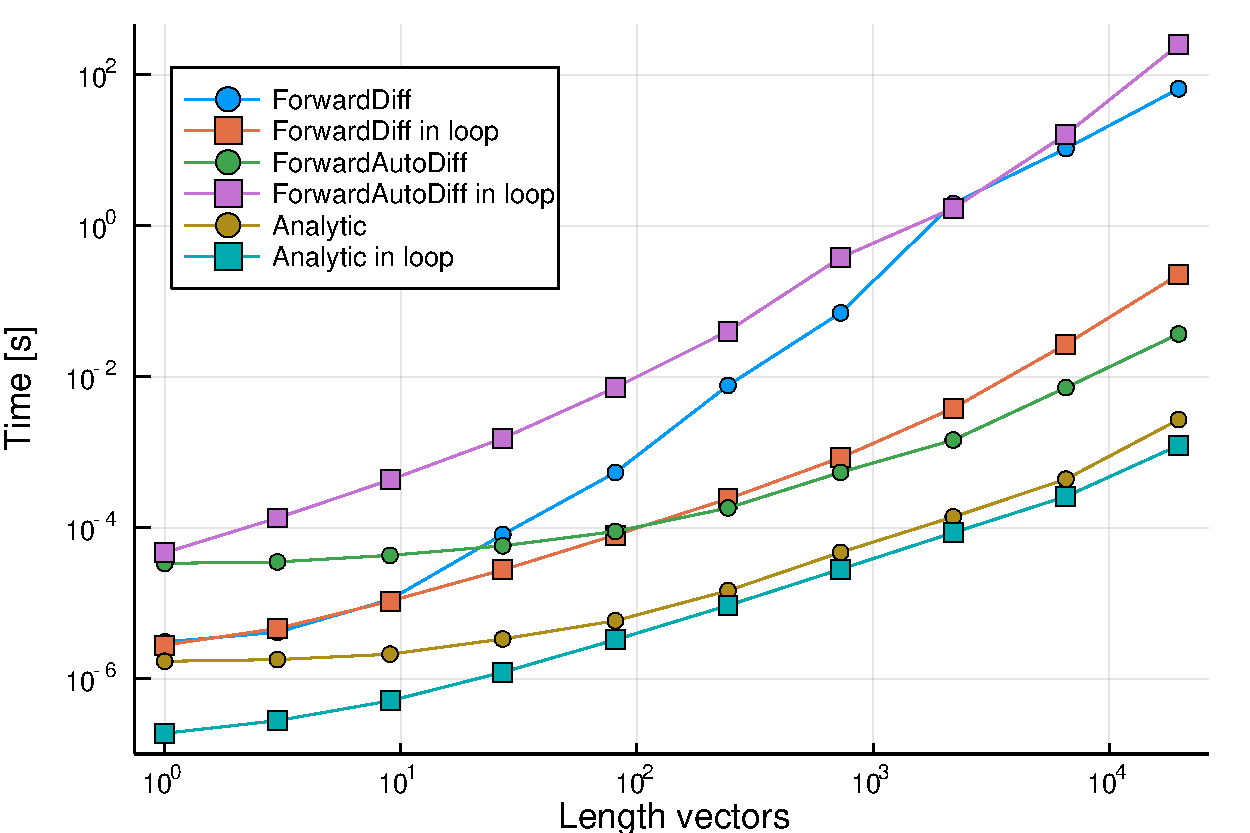
\includegraphics[width = 0.9\textwidth]{figures/benchmark_ad_in_loop.pdf}
    \caption{Computational time for calculating the value and gradient of $f$ in Equation \eqref{eq:benchmarkFunction} as                         a function of length of the input vectors.}
    \label{fig:benchmarkADInLoop}
\end{figure}

The first observation to make is that the \textit{ForwardAutoDiff} implementation is clearly not optimized for evaluating the vector function scalar by scalar, as it is the slowest method tested so far for all vector lengths. The next interesting observation is that Julia's implementation of AD, \textit{ForwardDiff}, can be made much more efficient in the evaluation of the vector function, by evaluating the function scalar by scalar. Using the method in \texttt{benchmarkADinLoop} with \textit{ForwardDiff}, we almost achieve the same test results as the regular \textit{ForwardAutoDiff} for long vectors. Although, it is important to mention that with the approach in \texttt{benchmarkADinLoop}, only the gradient of the function is obtained -- not the Jacobian. This limits the applicability of the method. In the particular case of the function $f$ in Equation \eqref{eq:benchmarkFunction}, the Jacobian will only be a diagonal matrix with the gradient of $f$ on the diagonal, but if we would evaluate a function like in Equation \eqref{eq:differenceFunction}, this approach would not work. Hence, although we almost manage to obtain the same performance in \textit{ForwardDiff} as we have in \textit{ForwardAutoDiff}, it comes with a cost that some types of functions cannot be evaluated. The implementation necessary to work around this and obtain the Jacobian with \textit{ForwardDiff} and \texttt{benchmarkADinLoop} will slow the computation down. For a vector function with large input vectors, \textit{ForwardAutoDiff} is therefore a better approach. 

Other than this, it is interesting to see that the evaluation of the analytical solution in a loop is faster than its vectorized counterpart. Here, Julia shows a real strength compared to MATLAB, where a function evaluation like the vector function $f$ will be much slower in a loop than with vector multiplication.
\begin{figure}[H]
    \centering
    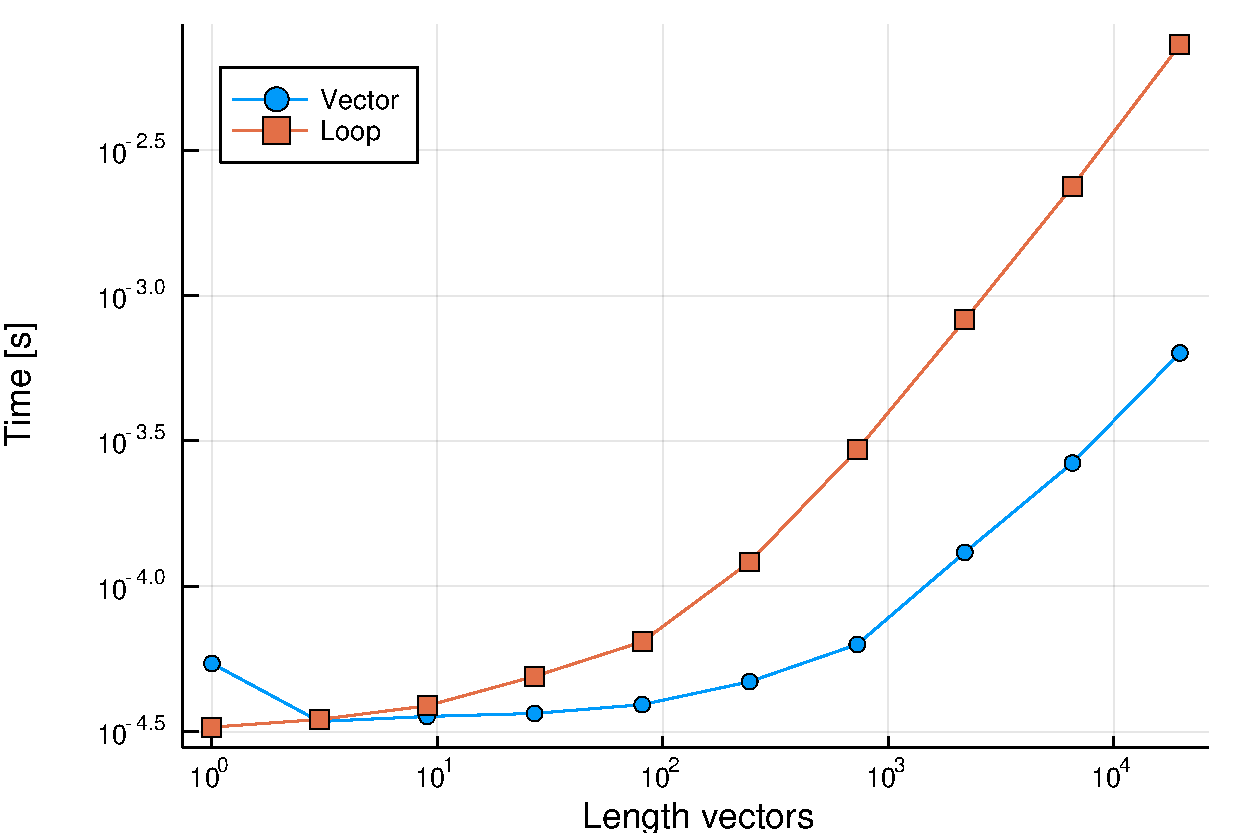
\includegraphics[width = 0.9\textwidth]{figures/benchmark_matlab_multiplication.pdf}
    \caption{Computational time for evaluating the analytic functions $f$, $f_x$, $f_y$ and $f_z$ from \eqref{eq:benchmarkFunction} as a function of length of the input vectors in MATLAB.}
    \label{fig:matlabMultiplication}
\end{figure}
\autoref{fig:matlabMultiplication} shows how much time MATLAB uses to evaluate the analytic functions $f$, $f_x$, $f_y$ and $f_z$ from Equation \eqref{eq:benchmarkFunction} as vector multiplication and in a for-loop. The analytic graphs in \autoref{fig:benchmarkADInLoop} demonstrates the time Julia uses to evaluate the same functions. Where the vector multiplication and for-loop scale equally good in Julia, and the for-loop actually perform better, MATLAB's for-loops scale much worse than the vector multiplication in contrast. This can be viewed as a first indication that the developers of Julia actually have managed to create a language with similar mathematical syntax as MATLAB and the computational efficiency of C.